\chapter{对向量的介绍}

\section{Vector}

\begin{definition}[Vector]
    一个有序的数字列表.

    \( \left[\begin{array}{c}-1.1 \\ 0.0 \\ 3.6 \\ -7.2\end{array}\right] \) 或者 \( \quad\left(\begin{array}{c}-1.1 \\ 0.0 \\ 3.6 \\ -7.2\end{array}\right) \) 或者 \( \quad(-1.1,0,3.6,-7.2) \)
\end{definition}

表中的数字是\textit{元素}(\textit{项、系数、分量}). 元素的数量是向量的\textit{大小}(\textit{维数,长度}). 大小为n的向量称为\textit{$n$维向量}. 
向量中的数字通常被称作\textit{标量}. 

用符号来表示向量,比如$\alpha$ ,$b$,一般小写字母表示. 其它表示形式 $\boldsymbol{g}, \vec{a}$

\begin{definition}[n维向量 \( a \) 的第 \( i \) 元素]
    n维向量 \( a \) 的第i \( i \) 元素表示为 \( a_{i} \).

    有时i指的是向量列表中的第i个向量.
\end{definition}

\begin{definition}[$a=b$]
    对于所有$i$,如果有$a_i = b_i$,则称两个相同大小的向量$a$和$b$是相等的,可写成$a = b$
\end{definition}

\begin{definition}[stacked vector]
    假设$b$、$c$、$d$是大小为$m$、$n$、$p$的向量
    
    $$ a=\left[\begin{array}{l}b \\ c \\ d\end{array}\right] $$

    $$ a=\left(b_{1}, b_{2}, \ldots, b_{m}, c_{1}, c_{2}, \ldots, c_{n}, d_{1}, d_{2}, \ldots, d_{p}\right) $$
\end{definition}

\begin{definition}[零向量]
    所有项为0的n维向量表示为$0_n$或者$0$.
\end{definition}

\begin{definition}[全一向量]
      所有项为1的n维向量表示为$\boldsymbol{1}_n$或者$1$.
\end{definition}

\begin{definition}[单位向量]
    当第i项为1,其余项为0时表示为$e_i$

    $$ {e}_{1}=\left[\begin{array}{l}1 \\ 0 \\ 0\end{array}\right], \quad e_{2}=\left[\begin{array}{l}0 \\ 1 \\ 0\end{array}\right], \quad e_{3}=\left[\begin{array}{l}0 \\ 0 \\ 1\end{array}\right] $$
\end{definition}

\begin{definition}[稀疏向量]
    如果一个向量的许多项都是0,该向量为稀疏(Sparse)的. 稀疏向量能在计算机上高效地存储和操作. 

$\operatorname{nnz}(x)$是指向量$x$中非零的项数(number of non-zeros),有时用 $\ell_0$表示 . 

\end{definition}

向量 \( x=\left(x_{1}, x_{2}\right) \) 可以在二维中表示一个位置或一个位移、 图像、 单词统计、颜色等. 

\section{Vector Space}

\begin{definition}[向量空间$V$]
    设 \( V \) 是非空子集, \( P \) 是一数域, 向量空间$V$满足:

    \begin{enumerate}
        \item 向量加法: \( V+V \rightarrow V \), 记作 \( \forall x, y \in V \), 则 \( x+y \in V( \) 加法封闭)
        \item 标量乘法: \( F \times V \rightarrow V \), 记作 \( \forall x \in V, \lambda \in P \), 则 \( \lambda x \in V( \) 乘法封闭)
    \end{enumerate}

上述两个运算满足下列八条规则 \( (\forall x, y, z \in V, \lambda, \mu \in P) \) 
\begin{enumerate}
    \item \( x+y=y+x \) (交换律) 
    \item \( x+(y+z)=(x+y)+z \) (结合律)
    \item \( V \) 存在一个零元素, 记作0, \( x+0=x \)
    \item 存在 \( x \) 的负元素,记作 \( -x \), 满足 \( x+(-x)=0 \)
    \item \( \forall x \in V \), 都有 \( 1 x=x, 1 \in P \)
    \item \( \lambda(\mu x)=(\lambda \mu) x \)
    \item \( (\lambda+\mu) x=\lambda x+\mu x \)
    \item \(  \lambda(x+y)=\lambda x+\lambda y \)
\end{enumerate}
\end{definition}

\begin{corollary}
    向量空间也称为线性空间.
\end{corollary}

\begin{corollary}
    如果 \( x, y \in \mathbb{R}^{2} \), 则 \( x+y \in \mathbb{R}^{2}, \lambda x \in \mathbb{R}^{2}(\lambda \in \mathbb{R}) \).
\end{corollary}

\begin{definition}[数域]
    数的非空集合$P$,且其中任意两个数的和、差、积、商(除数不为零)仍属于该集合,则称数集$P$为一个数域. 
\end{definition}

\begin{example}
    有理数 $ \mathbb{Q} $
\end{example}

\begin{example}
    实数 $ \mathbb{R} $

    $ x, y \in \mathbb{R}, x=1, y=2 $
    $ x+y \in \mathbb{R}  ,x \times y \in \mathbb{R} $
\end{example}

\begin{example}
    复数 $ \mathbb{C} $
\end{example}

\section{向量运算}

\begin{definition}[向量加法]
    $n$维向量$a$和$b$可以相加,求和形式表示为$a + b$.

    设向量 \( a, {b}, {C} \) 是向量空间 \( V \) 的元素,即 \( a, {b}, {c} \in V_{\text {.  }} \)

\begin{enumerate}
    \item 交换律: \( a+b=b+a \)
    \item 结合律: \( (a+b)+c=a+(b+c) \) (因此可写成 \( a+{b}+{c}) \)
    \item \( a+0=0+a=a \)
    \item \( a-a=0 \)
\end{enumerate}
\end{definition}

\begin{corollary}[向量位移相加]
    如果二维向量$a$和$b$都表示位移,则它们的位移之和为$a + b$
\end{corollary}

\begin{example}
    点$q$到点$p$的位移是$p-q$.

    

\tikzset{every picture/.style={line width=0.75pt}} %set default line width to 0.75pt        

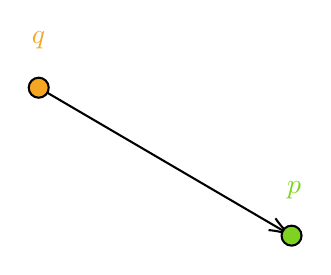
\begin{tikzpicture}[x=0.75pt,y=0.75pt,yscale=-1,xscale=1]
%uncomment if require: \path (0,300); %set diagram left start at 0, and has height of 300

%Straight Lines [id:da6747700231115574] 
\draw    (104.82,116.82) -- (224.91,187.09) ;
\draw [shift={(226.64,188.1)}, rotate = 210.34] [color={rgb, 255:red, 0; green, 0; blue, 0 }  ][line width=0.75]    (10.93,-3.29) .. controls (6.95,-1.4) and (3.31,-0.3) .. (0,0) .. controls (3.31,0.3) and (6.95,1.4) .. (10.93,3.29)   ;
%Shape: Circle [id:dp2346779756728088] 
\draw  [fill={rgb, 255:red, 126; green, 211; blue, 33 }  ,fill opacity=1 ] (221.82,188.1) .. controls (221.82,185.44) and (223.97,183.29) .. (226.64,183.29) .. controls (229.3,183.29) and (231.45,185.44) .. (231.45,188.1) .. controls (231.45,190.76) and (229.3,192.92) .. (226.64,192.92) .. controls (223.97,192.92) and (221.82,190.76) .. (221.82,188.1) -- cycle ;
%Shape: Circle [id:dp32683820972368327] 
\draw  [fill={rgb, 255:red, 245; green, 166; blue, 35 }  ,fill opacity=1 ] (100,116.82) .. controls (100,114.16) and (102.16,112) .. (104.82,112) .. controls (107.48,112) and (109.64,114.16) .. (109.64,116.82) .. controls (109.64,119.48) and (107.48,121.64) .. (104.82,121.64) .. controls (102.16,121.64) and (100,119.48) .. (100,116.82) -- cycle ;

% Text Node
\draw (100,88.4) node [anchor=north west][inner sep=0.75pt]  [color={rgb, 255:red, 245; green, 166; blue, 35 }  ,opacity=1 ]  {$q$};
% Text Node
\draw (223,160.4) node [anchor=north west][inner sep=0.75pt]  [color={rgb, 255:red, 126; green, 211; blue, 33 }  ,opacity=1 ]  {$p$};


\end{tikzpicture}

\end{example}

\begin{definition}[标量与向量的乘法]
    $$ \beta a=\left[\begin{array}{c}\beta a_{1} \\ \vdots \\ \beta a_{n}\end{array}\right] $$

    标量 \( \beta, \gamma \) 与向量 \( a 、 b \)进行乘法, 有如下性质:
\begin{enumerate}
    \item 结合律: \( (\beta \gamma) a=\beta(\gamma a) \)
    \item 左分配律: \( (\beta+\gamma) a=\beta a+\gamma a \)
    \item 右分配律: \( \beta(a+b)=\beta a+\beta b \)
\end{enumerate}
\end{definition}

\begin{definition}[线性组合]
    对于向量 \( a_{1}, \ldots, a_{m} \) 和标量 \( \beta_{1}, \ldots, \beta_{m} \),
    $$ \beta_{1} a_{1}+\cdots+\beta_{m} a_{m} $$
    是向量的线性组合. \( \beta_{1}, \ldots, \beta_{m} \) 是该向量的\textit{系数}. 
\end{definition}

\begin{example}
    对于任何向量 \( b \in \mathbb{R}^{n} \), 有如下等式
    $$ b=b_{1} e_{1}+\cdots+b_{n} e_{n}, b=\left[\begin{array}{c}b_{1} \\ b_{2} \\ \vdots \\ b_{n}\end{array}\right] $$
\end{example}

\section{内积}

\begin{definition}[内积]
    在数域 \( \mathbb{R} \) 上的向量空间 \( V \), 定义函数 \( \langle\cdot,\cdot\rangle:V \times V \rightarrow \mathbb{R} \), 满足:

    \begin{enumerate}
        \item $ \langle{a}, {a}\rangle \geq 0, \forall {a} \in V $, 当且仅当 $a=0$ 时 $ \langle a, a\rangle=0 $
        \item \( \langle\alpha {a}+\beta {b}, c\rangle=\alpha\langle{a}, c\rangle+\beta\langle{b}, c\rangle, \forall \alpha, \beta \in \mathbb{R} \), 且 \( {a}, {b}, c \in V \)
        \item \( \langle{a}, {b}\rangle=\langle{b}, {a}\rangle, \forall {a}, {b} \in V \)
    \end{enumerate}

    函数 \( \langle\cdot,\cdot\rangle:V \times V \rightarrow \mathbb{R} \)成为内积. 
\end{definition}

\begin{example}
    在向量空间 \( \mathbb{R}^{n} \) 上, 计算两个向量对应项相乘之后求和函数
    \[ \langle a, b\rangle=a_{1} b_{1}+a_{2} b_{2}+\cdots+a_{n} b_{n}=a^{T}_{b} \]

where \( a=\left[\begin{array}{c}a_{1} \\ a_{2} \\ \vdots \\ a_{n}\end{array}\right], b=\left[\begin{array}{c}b_{1} \\ b_{2} \\ \vdots \\ b_{n}\end{array}\right] \in \mathbb{R}^{n} \).
\end{example}

\begin{proof}
    \( \langle a, a\rangle=a_{1} a_{1}+a_{2} a_{2}+\cdots+a_{n} a_{n}=\sum_{i=1}^{n} a_{i}^{2} \geq 0,\langle a, a\rangle=0 \), 则 \( a=0 \)

    $$\begin{aligned} \langle\alpha a+\beta {b}, {c}\rangle &=\left(\alpha a_{1}+\beta b_{1}\right) c_{1}+\left(\alpha a_{2}+\beta b_{2}\right) c_{2}+\cdots+\left(\alpha a_{n}+\beta b_{n}\right) c_{n} 
    \\ &=\alpha \sum_{i=1}^{n} a_{i} c_{i}+\beta \sum_{i=1}^{n} b_{i} c_{i}
    \\ &=\alpha\langle a, c\rangle+\beta\langle b, c\rangle\end{aligned} $$

    $$ \langle a, b\rangle=a^{{T}} b=b^{{T}} a=\langle b, a\rangle $$
\end{proof}

内积的性质:交换律、结合律、分配律. 

交换律: \( a^{T} b=b^{T} a \)

结合律: \( (\gamma a)^{T} b=\gamma\left(a^{T} b\right) \)

分配律: \( (a+b)^{T} c=a^{T} c+b^{T} c \)

\subsection{常用的内积等式}
\begin{corollary}[选出第$i$项]
    $$ e_{i}^{T} a=a_{i} $$
\end{corollary}

\begin{corollary}[向量每一项之和]
    $$ \mathbf{1}^{T} a=a_{1}+\cdots+a_{n} $$
\end{corollary}

\begin{corollary}[向量每一项的平方和]
    $$ a^{T} a=a_{1}^{2}+\cdots+a_{n}^{2} $$
\end{corollary}

\begin{corollary}[向量元素的平均值]
    $$ (\mathbf{1} / n)^{T} a=\left(a_{1}+\cdots+a_{n}\right) / n $$
\end{corollary}

\begin{corollary}[Selective sum]
    Let $ b $ be a vector all of whose entries are either 0 or 1 . Then $$ b^{T} a $$ is the sum of the elements in $ a $ for which $ b_{i}=1 $.
\end{corollary}

\begin{definition}[The sum of block vectors]
    If the vectors $ a $ and $ b $ are block vectors, and the corresponding blocks have the same sizes (in which case we say they \textit{conform}), then 

    $$ a^{T} b=\left[\begin{array}{c}a_{1} \\ \vdots \\ a_{k}\end{array}\right]^{T}\left[\begin{array}{c}b_{1} \\ \vdots \\ b_{k}\end{array}\right]=a_{1}^{T} b_{1}+\cdots+a_{k}^{T} b_{k} $$
\end{definition}

内积用途很广.

\begin{example}[计算同时出现的项目数]
   $$
a=(0,1,1,1,1,1,1), \quad b=(1,0,1,0,1,0,0)
$$
Here we have $ a^{T} b=2 $, which is the number of objects in both $ A $ and $ B $ (i.e., objects 3 and 5). 
\end{example}

\begin{example}[Weights, features, and score]
    When the vector $f$ represents a set of \textit{features} of
    an object, and $w$ is a vector of the same size (often called a \textit{weight vector} ), the
    inner product $w^T f$ is the sum of the feature values, scaled (or weighted) by
    the weights, and is sometimes called a \textit{score}.
\end{example}

\begin{example}
    $$ p(x)=c_{1}+c_{2} x+\cdots+c_{n-1} x^{n-2}+c_{n} x^{n-1} $$

    Let $t$ be a number, $ z=\left(1, t, t^{2}, \ldots, t^{n-1}\right) $  be the $n$-vector of powers
    of $t$. Then

    $$ c^{T} z=p(t) $$
\end{example}


\section{Cauchy-Schwartz Inequality}
\begin{theorem}[Cauchy-Schwartz Inequality]
    设 \( \langle \cdot,\cdot \rangle \) 是向量空间 \( V \) 上的内积, \( \forall x, y \in V \), 则有

    $$
|\langle x, y\rangle|^{2} \leq\langle x, x\rangle\langle y, y\rangle
$$
\end{theorem}

\begin{proof}
    令 \( \lambda \in \mathbb{R} \), 则有 \( 0 \leq\langle x+\lambda y, x+\lambda y\rangle \) \( =\langle x, x\rangle+\lambda\langle y, x\rangle+\lambda\langle x, y\rangle+\lambda^{2}\langle y, y\rangle \) \( =\langle x, x\rangle+2 \lambda\langle y, x\rangle+\lambda^{2}\langle y, y\rangle \) 
    
    则有 \( \lambda^{2}\langle y, y\rangle+2 \lambda\langle y, x\rangle+\langle x, x\rangle \geq 0, \forall \lambda \in \mathbb{R} . \)

    \( \nabla=(2\langle y, x\rangle)^{2}-4\langle y, y\rangle\langle x, x\rangle \leq 0 \)
    
\( |\langle x, y\rangle|^{2} \leq\langle x, x\rangle\langle y, y\rangle \)

当$ |\langle x, y\rangle|^{2}=\langle x, x\rangle\langle y, y\rangle $ 时, 有 $ \left\langle x, x\rangle^2 +2 \lambda\langle y, x\rangle+\lambda^{2}\langle y, y\rangle=0\right. $

也即 \( \langle x+\lambda y, x+\lambda y\rangle=0 \), 因此 \( x+\lambda y=0 \), 即 \( x=-\lambda y \).
\end{proof}

\section{浮点运算}

计算机以浮点格式存储(实)数值. 

基本的算术运算(加法,乘法等)被称为浮点运算(flop). 

算法或操作的时间复杂度:作为输入维数的函数所需要的浮点运算总数. 

算法复杂度通常以非常粗略地近似估算. 

(程序)执行时间的粗略估计:计算机速度/flops

目前的计算机大约是$1$Gflops/秒($10^9$flops/秒)

\begin{corollary}
    假设有$n$维向量$x$和$y$:

    \begin{itemize}
        \item $x+y$需要$n$次加法,所以时间复杂度为 ($n$)flops. 
        \item $x^T y$ 需要$n$次乘法和$n - 1$次加法,所以时间复杂度为$(2n - 1)$flops. 
        \item 对于$x^T y$,通常将其时间复杂度简化为$2n$,甚至为$n$. 
        \item 当$x$或$y$是稀疏的时候,算法的实际运算时间会比理论时间更少. 
    \end{itemize}
\end{corollary}



